\section{Introduction}

\subsection{Motivation}

\frame{
    \frametitle{Evolution of Web Data}
    \begin{figure}
        \centering
        \begin{subfigure}{.2\textwidth}
            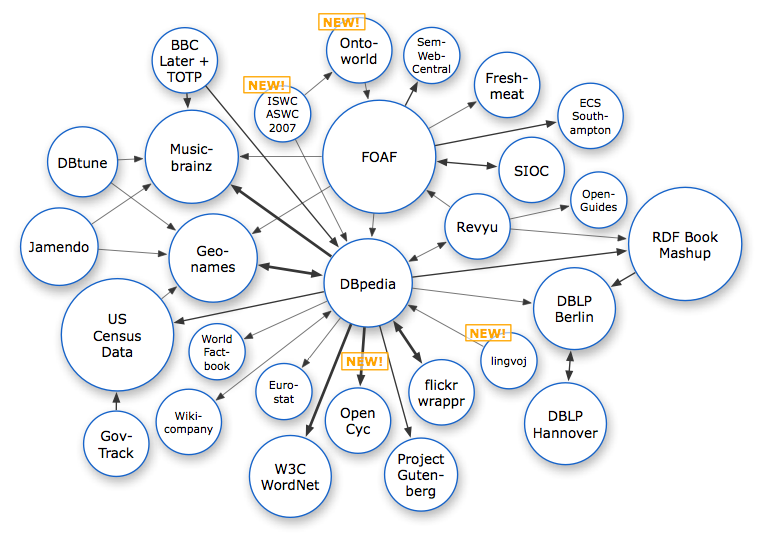
\includegraphics[width=\textwidth]{images/introduction/lod-cloud-2007-11-07}
        \end{subfigure}
        \begin{subfigure}{.215\textwidth}
            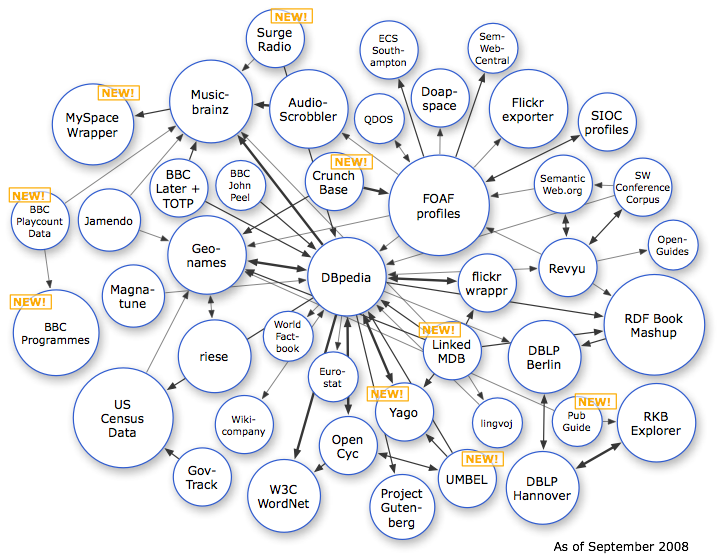
\includegraphics[width=\textwidth]{images/introduction/lod-cloud-2008-09-18}
        \end{subfigure}
        \begin{subfigure}{.225\textwidth}
            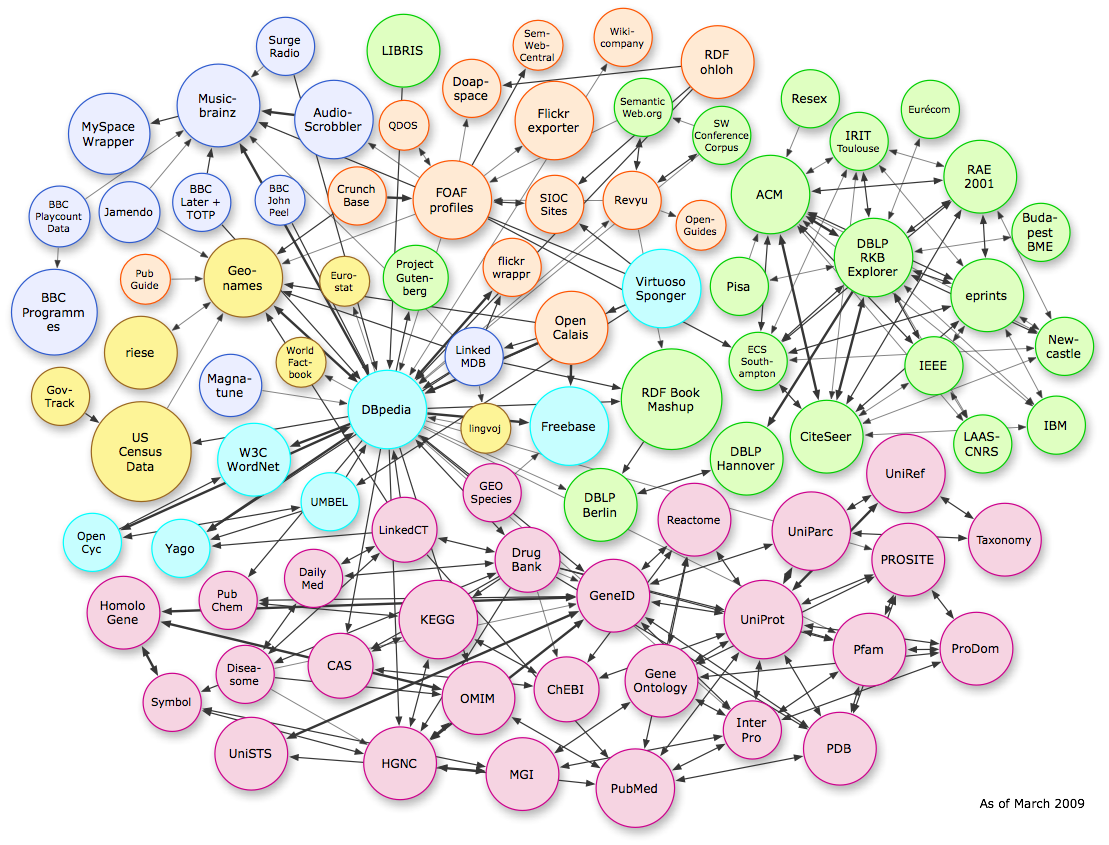
\includegraphics[width=\textwidth]{images/introduction/lod-cloud-2009-03-05}
        \end{subfigure}
        \begin{subfigure}{.325\textwidth}
            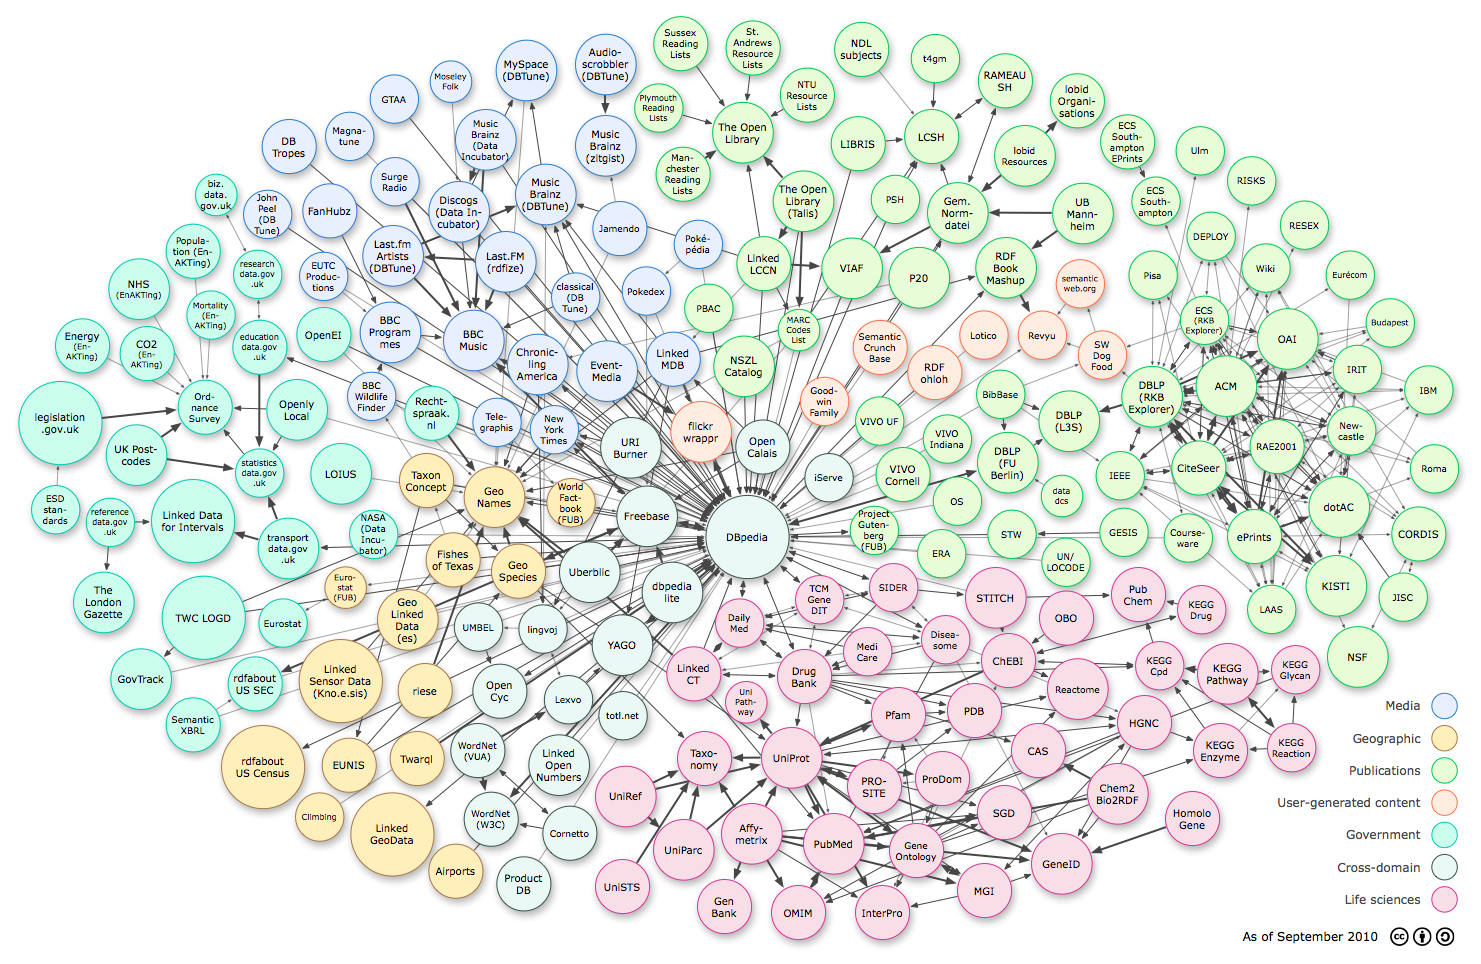
\includegraphics[width=\textwidth]{images/introduction/lod-cloud-2010-09-22}
        \end{subfigure}
        \begin{subfigure}{.365\textwidth}
            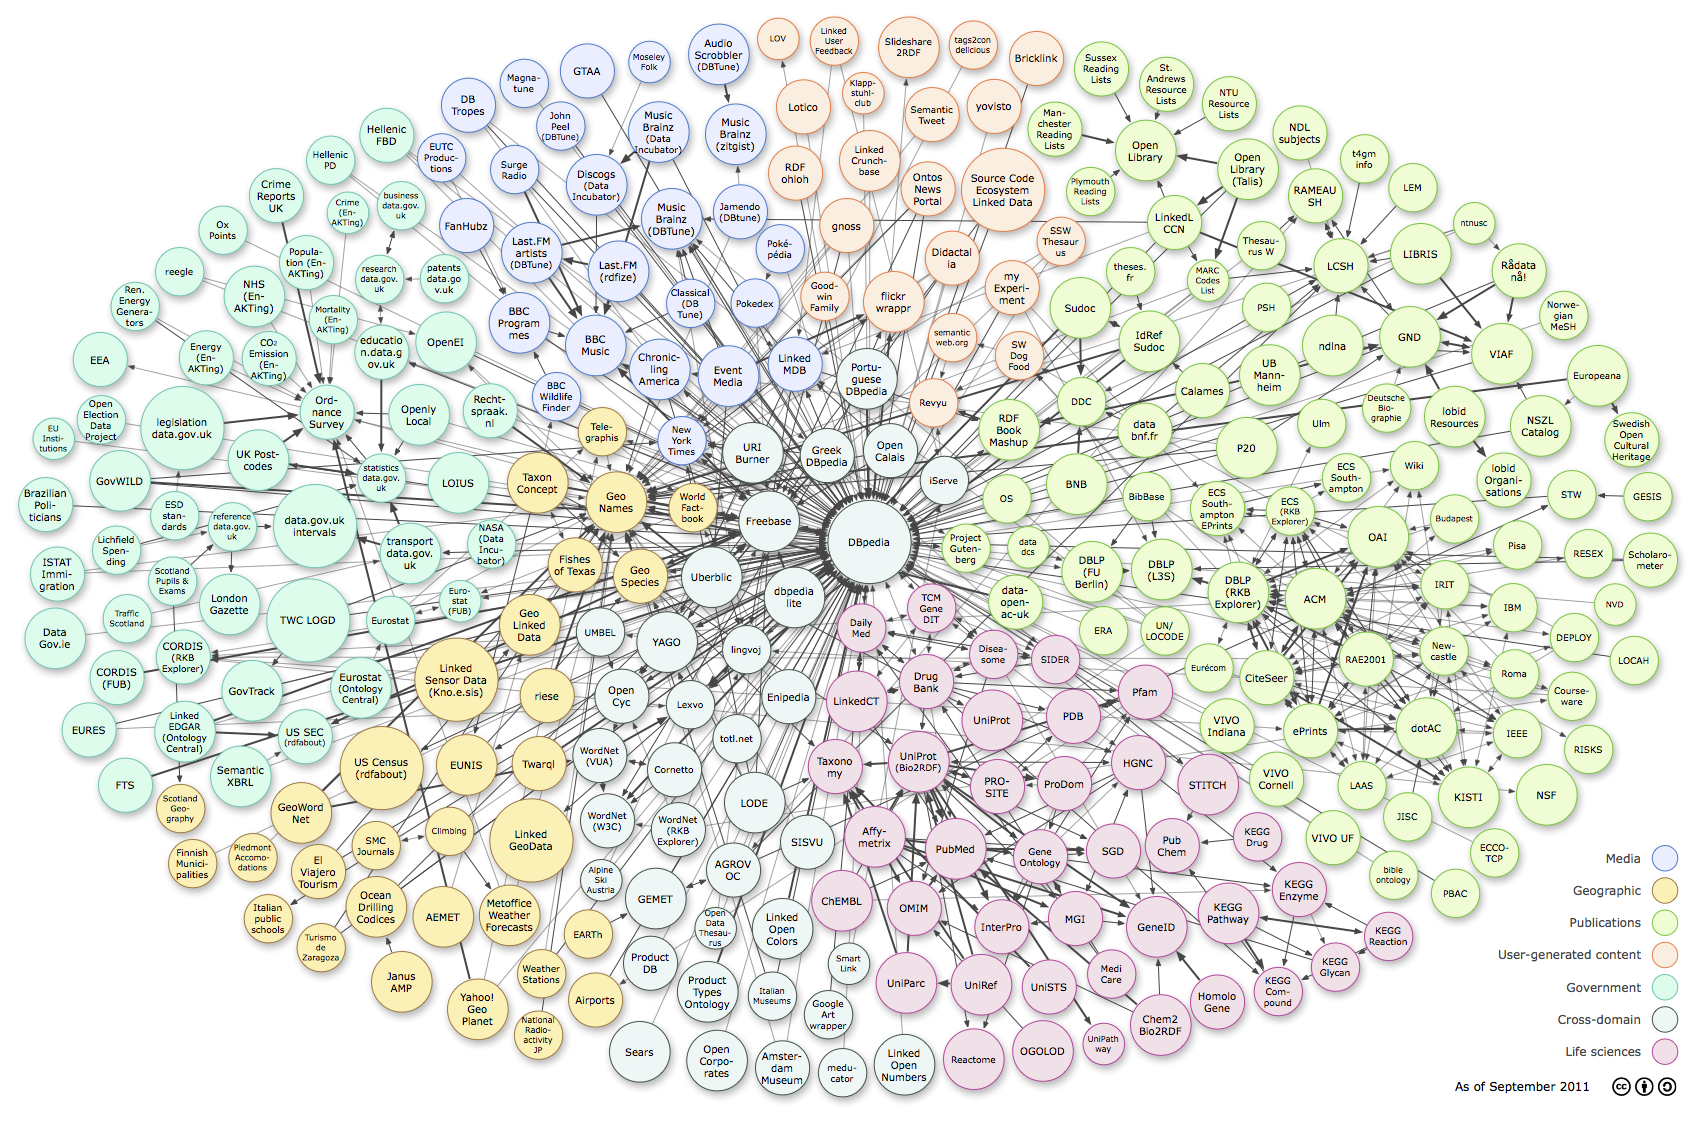
\includegraphics[width=\textwidth]{images/introduction/lod-cloud-2011-09-19}
        \end{subfigure}
        \begin{subfigure}{.45\textwidth}
            \includegraphics[width=\textwidth]{images/introduction/lod-cloud-2014-08-30}
        \end{subfigure}
    \end{figure}

    {\tiny Linking Open Data cloud diagrams 2008-2014, by Max Schmachtenberg, Christian Bizer, Anja Jentzsch and Richard Cyganiak. \url{http://lod-cloud.net/}}
}

%\frame{
    %\frametitle{How to Discover and Consume Web Data ?}
    %\begin{columns}[c]
        %\column{.5\textwidth}
        %\begin{block}{Accessing Information}
            %\begin{itemize}
                %\item Usefulness of Web Data is measured by the ease-of-access to the data
                %\item Relevant results to one's information need
            %\end{itemize}
        %\end{block}

        %\column{.5\textwidth}
        %\begin{block}{Obstacles}
            %\begin{itemize}
                %\item Structure and vocabulary of the data change over time
                %\item Schema is generally unknown
            %\end{itemize}
        %\end{block}
    %\end{columns}
%}

\frame{
    \frametitle{Creation of a Schema-like Data Structure}
    \begin{block}{Top-Down Schema: Ontologies}
        \begin{itemize}
            \item Data has a known structure\ldots
            \item \ldots but it does not keep up with the pace of Web Data evolution
        \end{itemize}
    \end{block}
    \uncover<2->{
        \begin{block}{Bottom-Up Schema: Graph Summarisation}
            \begin{itemize}
                \item Embraces the Semantic Web vision\ldots
                \item \ldots but is sensitive to data quality
            \end{itemize}
        \end{block}
    }
}

%\subsection{Use Case}

%\frame{
    %\frametitle{Use Case: Assisted Query Editing}
    %\begin{figure}
        %\centering
        %\resizebox{.9\textwidth}{!}{
            %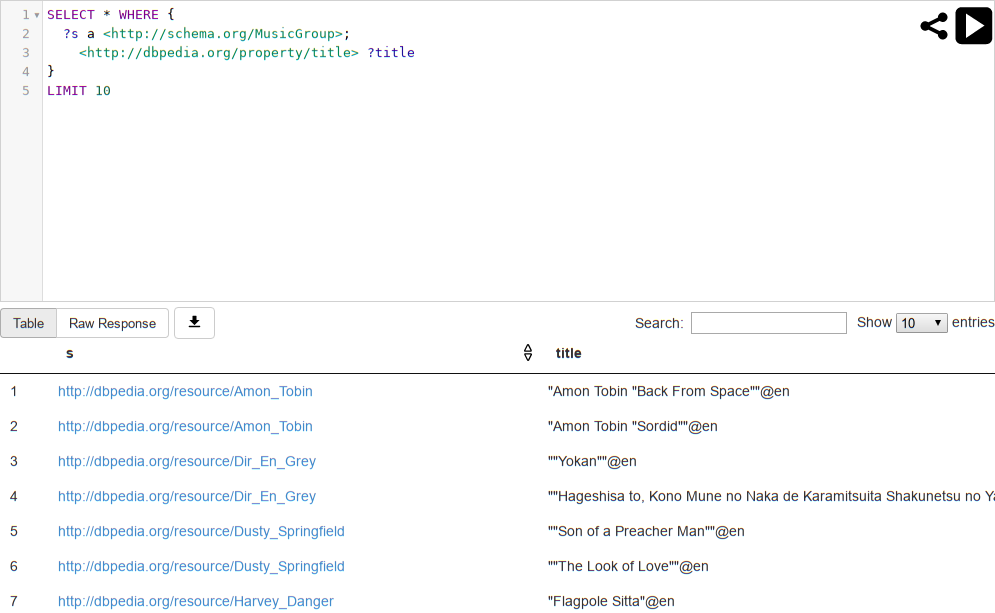
\includegraphics[scale=1]{images/introduction/use-case}
        %}
    %\end{figure}
%}

\subsection{Challenges}

\frame{
    \frametitle{Challenges}
    \begin{block}{Graph Summarisation}
        \begin{itemize}
            \item How to generate a description of a dataset ?
            \item Scale to billions of triples
            \item How to measure the precision of the generated output ?
        \end{itemize}
    \end{block}
}
%% vim: et:sw=4
